% !TeX root = ../main.tex

\chapter{CE$\nu$NS探测研究背景}

\section{CE$\nu$NS过程}

\begin{figure}
    \centering
    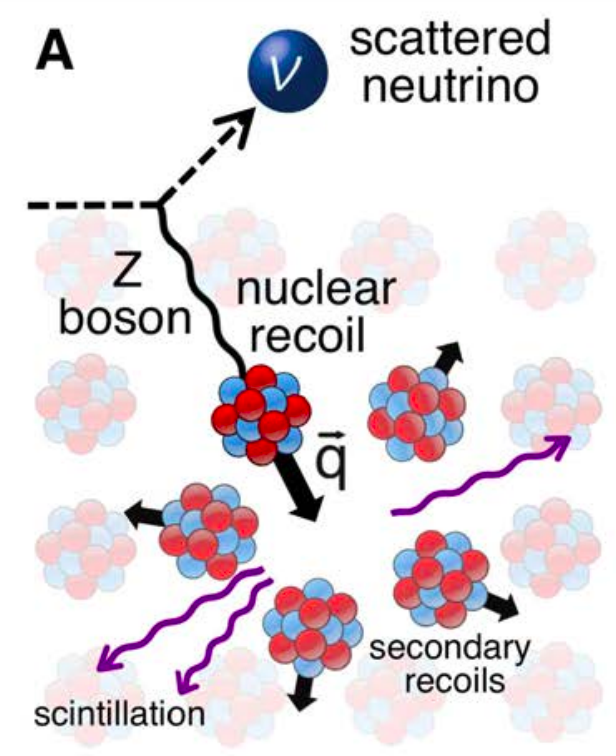
\includegraphics[width=0.4\linewidth]{figures/CEvNS_demo.png}
    \caption{中微子-原子核相干弹性散射示意图。中微子与原子核交换Z玻色子,同时也交换能量动量,产生核反冲(nuclear recoil, NR)。
    被加速的原子核以散射光(scintillation)和后续碰撞(secondary recoils)的形式继续将能量沉积到周围的物质中,
    最终这些信号被探测器记录到\cite{akimov_observation_2017}。}
    \label{fig:cevns_demo}
\end{figure}

CE$\nu$NS是中微子和原子核之间的弹性中性流相互作用,于1974年被首次预言提出\cite{freedman_coherent_1974,}。如图\ref{fig:cevns_demo}在中微子和原子核交换Z玻色子的过程中,若动量转移足够小,
则原子核近似作为一个整体与中微子作用,作用截面近似与原子核中的中子个数的平方成正比关系。

\begin{align}
    \label{eq:cevns}
    \frac{\mathrm{d}\sigma}{\mathrm{d}T} &= \frac{G_F^2 M}{2\pi}\left[(G_V+G_A)^2+(G_V-G_A)^2(1-\frac{T}{E_{\nu}})^2-(G_V^2-G_A^2)\frac{MT}{E_{\nu}^2}\right] \\
    G_V &= (g_V^p Z+g_V^n N)F^V(Q^2) \\
    G_A &= (g_A^p(Z_{+}-Z_{-})+g_A^n(N_{+}-N_{-}))F^A(Q^2) \\
    g_V^p &= \rho_{\nu N}^{NC}(\frac{1}{2} - 2\hat{\kappa}_{\nu N}\sin^2\theta_W) + 2\lambda^{uL} + 2\lambda^{uR} + \lambda^{dL} + \lambda^{dR} \\
    g_V^n &= -\frac{1}{2}\rho_{\nu N}^{NC} + \lambda^{uL} + \lambda^{uR} + 2\lambda^{dL} + 2\lambda^{dR}
\end{align}

公式\ref*{eq:cevns}为具有特定能量$E_{\nu}$的电子反中微子与特定质量$M$的原子核的CE$\nu$NS微分截面,
其中$T$为末态原子核动能,$G_F$为费米常数(Fermi constant),本文中取为1.1664$\times10^{-5}\si{GeV}^{-2}$,$Q$为动量转移,$Z$和$N$分别为原子核内质子和中子的个数。
$F^V$和$F^A$为形状因子,在低动量转移下可以认为$F^V(Q^2)=F^A(Q^2)=1$\cite{lewin_review_1996},
$\rho_{\nu N}^{NC},\hat{\kappa}_{\nu N}$为弱电理论参数,
$\lambda^{uL},\lambda^{uR},\lambda^{dL},\lambda^{dR}$是辐射校正参数\cite{barranco_probing_2005}。
$Z_{\pm}$和$N_{\pm}$是原子核内自旋(spin)取向为上($+$)和下($-$)的质子和中子个数。

经过计算,$|g_V^p|\ll|g_V^n|$,所以在 $G_V$ 参数中起主要作用的因素是中子个数 $N$;
另一方面,根据原子核物理理论,对于偶偶核(even-even nucleus),即原子核内质子数$Z$和中子数$N$均为偶数时,$Z_{+}=Z_{-},N_{+}=N_{-}$。
届时 $G_A=0$,我们可以利用这一点将CE$\nu$NS截面简化。

\begin{align}
    \label{eq:cevns_even_even}
    \frac{\mathrm{d}\sigma}{\mathrm{d}T} &= \frac{G_F^2 M}{2\pi}G_V^2\left[1+(1-\frac{T}{E_{\nu}})^2-\frac{MT}{E_{\nu}^2}\right] \\
    G_V &= (g_V^p Z+g_V^n N)F^V(Q^2)
\end{align}

公式\ref{eq:cevns_even_even}为CE$\nu$NS截面的的偶偶核简化形式。考虑到 $|g_V^p|\ll|g_V^n|$,则$G_V^2\approx N^2$,
最后可以近似得到$\frac{\mathrm{d}\sigma}{\mathrm{d}T}\approx N^2$,对于非偶偶核,该式也近似成立。这正是CE$\nu$NS相干性的体现。

对于不同种类的核素,因为原子核的质量$M$不同,所以微分截面$\frac{\mathrm{d}\sigma}{\mathrm{d}T}$不同。
将微分截面对原子核末态动能$T$积分,可以得到CE$\nu$NS总截面随着中微子能量$E_{\nu}$的变化关系。

\begin{figure}
    \centering
    \includesvg[width=0.6\linewidth]{figures/cross_section.svg}
    \caption{CE$\nu$NS对各种核素的截面随着中微子能量$E_{\nu}$的变化关系。作为对比,图中还包括了IBD\cite{akimov_observation_2017}的截面以及中微子-电子相干弹性散射(neutrino-electron elastic scattering, E$\nu$ES)的截面随着$E_{\nu}$的变化。几种截面都随着中微子能量升高而升高,但几种CE$\nu$NS截面始终高于IBD和与电子相互作用的截面。同时对于更重的元素,如$\mathrm{Xe}$,CE$\nu$NS截面相比于其他较轻元素更大。}
    \label{fig:xsec_elements}
\end{figure}

图\ref{fig:xsec_elements}中列举了几种探测器常用核素(元素)的CE$\nu$NS截面与$E_{\nu}$的关系。
从截面大小的角度看,CE$\nu$NS相比IBD更容易被探测;但是因为CE$\nu$NS的动量转移太小,且不同于IBD可以借助$\gamma$和中子进行事件标记,对CE$\nu$NS的成功探测远晚于IBD。
同时图\ref{fig:xsec_elements}也给提示我们选择探测器材料的思路:重元素的反应截面更大,对探测更有利。但是考虑到原子核末态动能也会随着元素质量数增加而偏向更低能量,
以及不同探测器介质下探测器技术和性能的差异,应综合考虑选择探测手段。

\section{CE$\nu$NS探测方法与进展}
